\documentclass[10pt,a4paper]{article}
\usepackage[margin=18mm]{geometry}
\usepackage[T1]{fontenc}
\usepackage{lmodern,microtype,graphicx,booktabs,amsmath}
\usepackage[font=small,labelfont=bf]{caption}
\usepackage{float}
\usepackage[hidelinks]{hyperref}
\usepackage{titlesec}
\setlength{\parindent}{0pt}
\setlength{\parskip}{5pt}
\titlespacing*{\section}{0pt}{9pt}{3pt}
\titleformat{\section}{\normalsize\bfseries}{\thesection}{.6em}{}
\graphicspath{{images/}}
\pagestyle{plain}
\begin{document}
\begin{center}
{\Large\bfseries Does verifier guidance improve coding accuracy?}
\end{center}
\vspace{-2mm}

We compared ordinary coding tools, optional verification, and instructed verification on Codeforces programming tasks. Across eight repetitions, instructed verification scored 85.50\% against the baseline's 82.50\%: $+3.00$ percentage points (pp), with a paired 97.5\% confidence interval (CI) of $[-0.38,\,+6.50]$. Optional access scored 81.38\%, a difference of $-1.13$ pp ($[-4.38,\,+2.13]$). Both intervals include zero; these data do not establish an accuracy improvement.

\section*{Design}
The benchmark contained 100 tasks: 50 rated 2000--2399 and 50 rated at least 2400 (range 2000--3500).\footnote{Task source: \url{https://github.com/dimativator/plsd-verifier-project}.} Each repetition evaluated every task in all three conditions. Eight repetitions produced 2,400 selected outcomes, 800 per condition. Runs used \texttt{gpt-5.6-luna} with medium reasoning in mini-SWE-agent 2.4.6.

The \textbf{baseline} used Python, shell tools and tests. \textbf{Optional} added CrossHair and a technical guide. CrossHair searches for violations of contracts written by the agent. \textbf{Instructed} provided the same guide but required relevant checks, interpretation of feedback, and repair or rechecking when useful. All conditions started from a blank Python file with the same task statements and tests. Each attempt allowed 100 agent steps, 600 seconds for solving and \$0.12 API cost.

\section*{Accuracy and cost}
Success means passing the retained private tests. Scores average the eight complete repetition scores. SD is their sample standard deviation; variance uses $n-1$ across repetitions (seven degrees of freedom).
\begin{center}
\small
\setlength{\tabcolsep}{6pt}
\begin{tabular}{lrrrrr}
\toprule
Condition & Score (\%) & SD (pp) & Variance (pp$^2$) & 95\% family CI (\%) & USD/task \\
\midrule
Baseline   & 82.50 & 1.69 & 2.86 & 76.75--87.75 & 0.01942 \\
Optional   & 81.38 & 3.11 & 9.70 & 75.75--86.75 & 0.01618 \\
Instructed & 85.50 & 1.69 & 2.86 & 79.88--90.63 & 0.01968 \\
\bottomrule
\end{tabular}
\end{center}
\vspace{-3mm}
\begin{figure}[H]
\centering
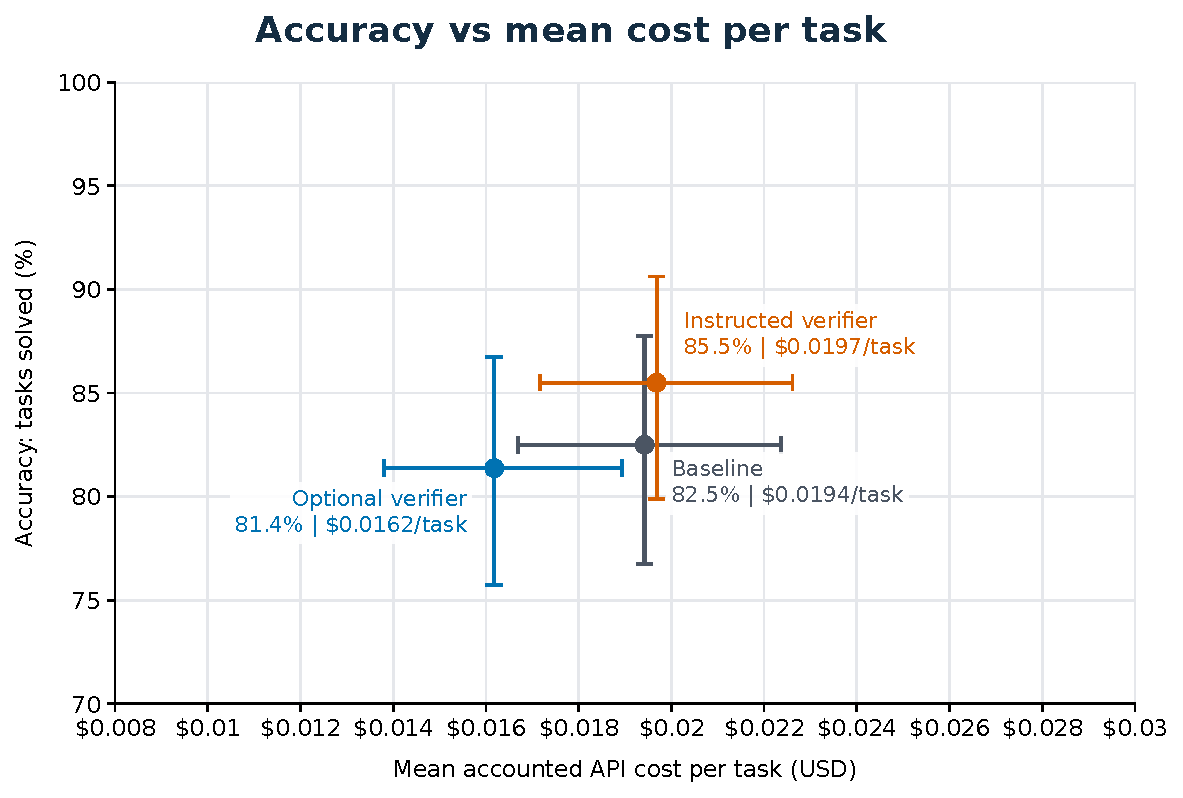
\includegraphics[width=0.88\linewidth]{accuracy-vs-cost.pdf}
\caption{Accuracy versus mean API cost per evaluation. Bars show marginal 95\% confidence intervals on both axes.}
\label{fig:accuracy-cost}
\end{figure}

\newpage
\section*{Planned study and exploratory extension}
Five repetitions were planned before collection. Their baseline, optional and instructed means were 83.0\%, 81.2\% and 85.4\%. The paired effects were optional $-1.8$ pp (97.5\% CI $[-5.6,\,+1.8]$) and instructed $+2.4$ pp ($[-1.2,\,+6.0]$). Three further repetitions were added after interim inspection, so the pooled eight-repetition analysis is exploratory. Neither analysis establishes an improvement.

\section*{Uncertainty}
Each problem is one task family. The intervals use 10,000 bootstrap draws, seed 20261123, sampling families within the two rating bands while keeping all repetitions and conditions together. Accuracy and cost use the same draws. Their marginal 95\% intervals are not a joint 95\% region. The two paired baseline comparisons use 97.5\% intervals, a Bonferroni adjustment for approximately 95\% familywise coverage.

These intervals describe performance on comparable task families. SD and variance instead describe repeated-run variation on this fixed benchmark. Eight repetitions still provide 100 task families, not 800 independent tasks per condition; the family intervals do not separately estimate model Monte Carlo uncertainty on this exact set.

\section*{Verifier use and cost}
Optional runs recorded no verifier invocation (0/800). Instructed runs recorded verifier use in 639/800 cases (79.9\%), including counterexample diagnostics in 106 runs and contract-confirmation diagnostics in 345; categories overlap. These observations show interaction with the verifier, but do not establish that its checks covered the task adequately. Optional access therefore tests offering a tool, while instructed verification tests the combined instruction-and-tool policy.

Total accounted API cost was \textbf{\$44.23}: \$15.54 baseline, \$12.94 optional and \$15.75 instructed. Mean cost divides each total by 800 evaluations. It includes 33 infrastructure replacements and their original attempts, and excludes preparation. Uncertain-delivery charges are retained conservatively; the plotted intervals describe variation between task families, not invoice uncertainty. Replacements do not add repetitions. Wrong answers and resource exits remain scored using the last saved program.

\section*{Limits}
This study covers one model, one verifier and one selection of 100 tasks. Passing the private tests is not a proof of correctness or complete Codeforces judge acceptance. The paired comparisons support the accuracy conclusions; overlapping separate arm intervals alone would not establish equivalence.

\vfill
{\footnotesize Evaluation date: 24 November 2026.}
\end{document}
